% Two ways to get the gradient back through a simulation.
% Compile: pdflatex adjoints.tex && pdftocairo -svg adjoints.pdf adjoints.svg
\documentclass[tikz,border=6pt]{standalone}
\usepackage{tikz}
\usepackage{amsmath}
\usepackage[T1]{fontenc}
\usetikzlibrary{arrows.meta,positioning,calc}

\definecolor{ink}{HTML}{2E2E2E}
\definecolor{greytx}{HTML}{7A7A7A}
\definecolor{fwd}{HTML}{3B6FB6}
\definecolor{revd}{HTML}{C0392B}
\definecolor{saved}{HTML}{2AA198}
\definecolor{panel}{HTML}{F4F6FA}

% #1 tag used in node names (must be letters/digits)  #2 y  #3 stored steps
\newcommand{\chain}[3]{%
  \foreach \i in {0,...,5}{%
    \node[draw=greytx,line width=0.8pt,fill=panel,rounded corners=3pt,
          minimum width=1.10cm,minimum height=0.76cm,text=ink,
          font=\sffamily\small] (#1\i) at ({\i*1.85},#2) {$a_\i$};}
  \foreach \i in {0,...,4}{%
    \pgfmathtruncatemacro{\j}{\i+1}
    \draw[-{Stealth[length=3pt]},fwd,line width=1pt]
          (#1\i) to[bend left=40] (#1\j);
    \draw[-{Stealth[length=3pt]},revd,line width=1pt,densely dashed]
          (#1\j) to[bend left=40] (#1\i);}
  \foreach \i in #3{%
    \node[draw=saved,line width=1.6pt,rounded corners=3pt,
          minimum width=1.10cm,minimum height=0.76cm] at ({\i*1.85},#2) {};}}

\begin{document}
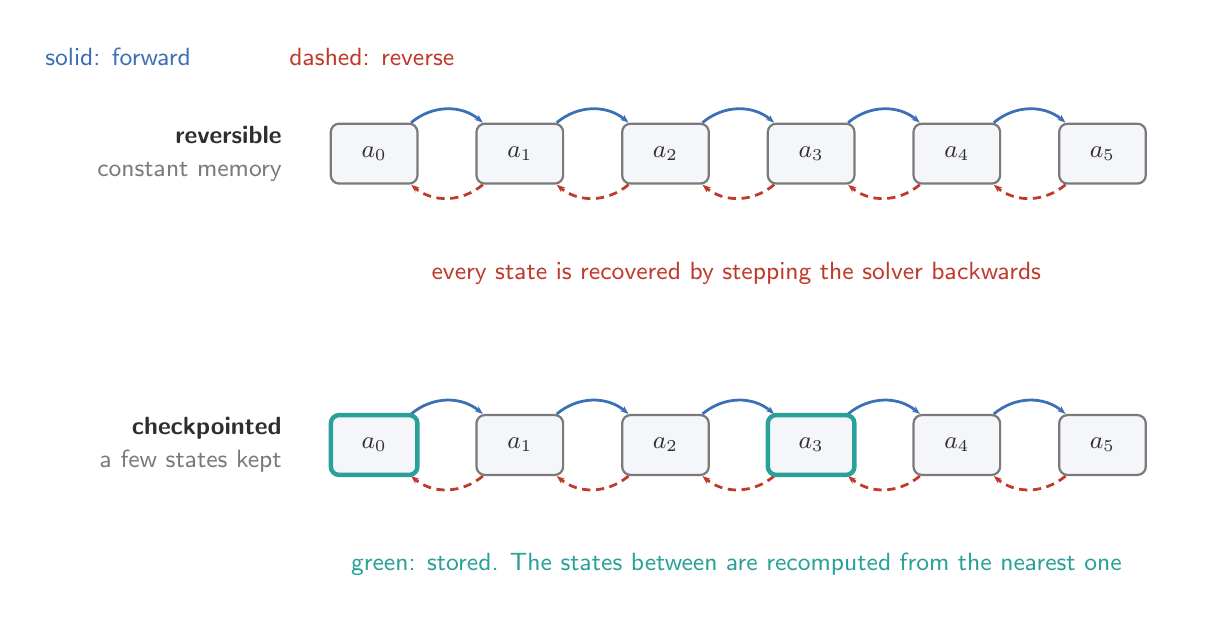
\begin{tikzpicture}[font=\sffamily]
  \useasboundingbox (-4.4,-4.6) rectangle (10.4,2.6);

  \chain{ra}{1.0}{{}}
  \node[anchor=east,align=right,text=ink,font=\sffamily\small] at (-1.05,1.0)
       {\textbf{reversible}\\[1pt]
        \textcolor{greytx}{\small constant memory}};
  \node[revd,font=\sffamily\small,anchor=north,align=center] at (4.6,-0.25)
       {every state is recovered by stepping the solver backwards};

  \chain{rb}{-2.7}{{0,3}}
  \node[anchor=east,align=right,text=ink,font=\sffamily\small] at (-1.05,-2.7)
       {\textbf{checkpointed}\\[1pt]
        \textcolor{greytx}{\small a few states kept}};
  \node[saved,font=\sffamily\small,anchor=north,align=center] at (4.6,-3.95)
       {green: stored. The states between are recomputed from the nearest one};

  \node[fwd,font=\sffamily\small,anchor=south west] at (-4.3,2.0)
       {solid: forward};
  \node[revd,font=\sffamily\small,anchor=south west] at (-1.2,2.0)
       {dashed: reverse};
\end{tikzpicture}
\end{document}
